%
% wavelets.tex
%
% (c) 2018 Prof Dr Andreas Müller, Hochschule Rapperswil
%
\section{Anwendung: Wavelets\label{section-wavelets}}
\rhead{Anwendung: Wavelets}
Die Erfindung der Fourier-Reihen durch Jean-Baptiste Fourier erm"oglichte,
beliebige periodische Funktionen in ihre Frequenzkomponenten zu zerlegen,
diese einzeln zu studieren, zu modifizieren und daraus eine neue Funktion
zu synthetisieren. Fourier-Reihen und die Fourier-Transformation haben
sich zu Standardwerkzeugen sowohl in den Anwendungen wie auch in der
reinen Mathematik entwickelt.

In der Praxis kennt man von einer Funktion, die zum Beispiel in
Oszilloskop misst, die Funktionswerte nur zu diskreten Zeitpunkten,
Abbildung~\ref{signal:vector}.
Auch von solchen Funktionen kann man das Frequenz-Spektrum bestimmen.
Die Theorie hat jedoch ein paar Nachteile:
\begin{compactenum}
\item Um die hochfrequenten Komponenten, also die ``Detailinformation''
"uber das Signal zu bekommen, muss man das gesamte Signal analysieren.
Man w"urde sich w"unschen, dass Detailinformationen aus einer Analyse
nur eines kurzen Zeitabschnitts des Signals ermittelbar sind.
\item "Andert man eine Frequenzkomponente, "andert sich das Signal
"uberall. Man w"urde sich w"unschen, dass "Anderungen m"oglichst nur
lokale Wirkung haben.
\end{compactenum}
Wavelets l"osen diese Probleme. Statt zeitlich ausgedehnter Sinus-
und Kosinus-Schwingungen werden nur kurze Wellenz"uge verwendet.
Je k"urzer sie sind, desto feiner die Details, die sie aus dem 
Signal analysieren. Leider ist es nicht ganz einfach, geeignete
Funktionen zu finden. Es muss viel mathematischer Aufwand getrieben
werden, damit die Wavelets m"oglichst glatt werden, nicht lange
dauern, und ausserdem das Signal m"oglichst so analysieren, dass
man damit auch praktisch n"utzliche Aufgaben l"osen kann.

Das Prinzip der Analyse eines Signals mit Wavelets kann jedoch
auch mit der Haar-Basis illustriert werden. Dies wird in diesem
Abschnitt unternommen.

\subsection{Signale}
\begin{figure}
\begin{center}
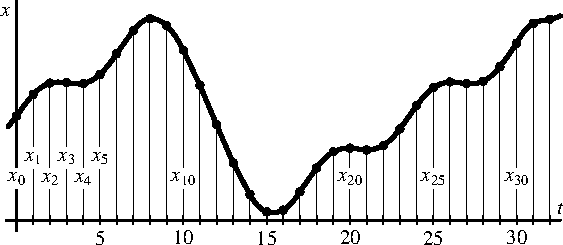
\includegraphics[width=0.9\hsize]{images/signal-1}
\end{center}
\caption{Sampling eines Signals\label{signal:vector}}
\end{figure}
Wir stellen uns ein Signal vor, welches zu einer grossen Zahl $N$
von Zeitpunkten mit gleichem Abstand abgetastet wird,
Abbildung~\ref{signal:vector}. Das Signal
wird dadurch zu einer Liste von Werten $x_1,x_1,\dots,x_N$, die
alles beinhalten, was wir "uber das Signal wissen. Ein Signal
ist also im wesentlichen ein Vektor
$$
x=\begin{pmatrix}x_1\\x_2\\\vdots\\x_N\end{pmatrix}
$$
Die Menge $\mathbb R^N$ dieser Vektoren bezeichnen wir in diesem
Kapitel mit $V$. 

Die "ublichen Operationen mit Vektoren haben eine naheliegende
"Ubersetzung f"ur Signale. Die Summe zweier Vektoren entspricht
der "Uberlagerung, die Multiplikation mit einem skalaren Faktor
entspricht einer Verst"arkung des Signals. 

Ein Skalarprodukt l"asst sich wie "ublich bilden, doch ziehen
wir folgende Definition vor:
$$
x\cdot y=\sum_{i=1}^Nx_iy_i
$$
Die Vektoren $e_i$ mit $1\le i\le N$ bilden nat"urlich immer noch
eine orthonormierte Basis, diese ist jedoch f"ur die Anwendungen
nicht unbedingt gut geeignet.

Wir schreiben die Komponenten dieser Vektoren auch $x(i)$ um
eine Schreibweise zu erhalten, die "ahnlich ist der Funktionsschreibweise
f"ur eine Zeitabh"angige Funktion.

\subsection{Anforderungen an eine Basis}
Die Standardbasis $e_i$ passt nicht zu der Art und Weise, wie ein
Ingenieur das Signal studiert. Der Standardbasis-Vektor $e_i$
entspricht einem Peak zur Zeit $i$, zu allen anderen Zeiten
ist der Signalwert $0$.
Ein Ingenieur wird sich das Signal
typischerweise bei verschiedenen zeitlichen Aufl"osungen
ansehen, indem er die Zeitbasis am Oszilloskop ver"andert.
Bei geringer Aufl"osung sind nur die niederfrequenten
Anteile des Signales sichtbar, bei hoher zeitlicher Aufl"osung
werden zus"atzliche Details sichtbar.
Gesucht ist daher eine Basis, die an solche Aufl"osungs"anderungen
angepasst ist.

Dem Ingenieur ist auch egal, wo innerhalb des Signals sich
ein bestimmtes Ereignis abspielt, die Basis sollte sich also
auch bei Verschiebungen entlang der Zeitachse nicht "andern.

Gesucht ist also eine alternative Basis aus Signalen, die
sich durch Zeitverschiebung und Skalierung ineinander "uberf"uhren
oder mindestens vergleichen lassen.

Die einfachsten Skalentransformationen, f"ur die wir die Basisvektoren
vorbereiten wollen, sind die zeitlichen Streckungen um den Faktor 2.
Dies wird nur m"oglich sein, wenn die Zahl $N$ gen"ugen durch $2$
teilbar ist, der Einfachheit halber setzen wir daher fest, dass
f"ur den Rest dieses Kapitels $N=2^k$.

Die Analyse eines Signals, die Zerlegung in Basisvektoren, erfordert
normalerweise die L"osung eines linearen Gleichungssystems.
Es ist unm"oglich, dies f"ur grosse Datenmengen in Echtzeit
durchzuf"uhren. Verwendet man aber eine orthonormierte Basis,
ist die Zerlegung einfach: die Koeffizienten entstehen einfach
durch Berechnung eines Skalarproduktes.

Gesucht ist jetzt also eine Basis mit folgenden Eigenschaften:
\begin{compactenum}
\item Ein Basisvektor geht in einen anderen Basisvektor "uber, wenn
man die Zeitachse um den Faktor 2 komprimiert.
\item Ein Basisvektor geht in einen anderen Basisvektor "uber, wenn
man ihn entlang der Zeitachse verschiebt, wenigstens f"ur
gewisse Offsets.
\item Die Vektoren sind orthonormiert.
\end{compactenum}
In den folgenden Abschnitten sollen diese Forderungen nach und
nach erf"ullt werden.

\subsection{Eine skaleninvariante Vektorfamilie}
Wir konstruieren jetzt eine Familie von Vektoren $\varphi_{i,j}$
wie folgt. $\varphi_{0,0}$ besteht aus lauter Einsen. In $\varphi_{1,j}$
ist die H"alfte der Komponenten $0$, die andere H"alfte hat den
Wert $1$. 
Diese Vektoren sind also:
\begin{align*}
\varphi_{0,0}&=\begin{pmatrix}1\\\vdots\\1\end{pmatrix}
\\
\varphi_{1,0}&=\begin{pmatrix}1\\\vdots\\1\\0\\\vdots\\0\end{pmatrix}&
\varphi_{1,1}&=\begin{pmatrix}0\\\vdots\\0\\1\\\vdots\\1\end{pmatrix}
\end{align*}
Siehe auch Abbildungen~\ref{wavelet-phi00} und \ref{wavelet-phi10-11}.
Diese Konstruktion l"asst sich fortsetzen:
\begin{align*}
\varphi_{i,j}(t)&=\begin{cases}
1&\qquad j2^{k-i}<t\le (j+1)2^{k-i}\\
0&\qquad\text{sonst}
\end{cases}
\end{align*}
Das Signal $\varphi_{i,j}$ ist also nur auf einem Abschnitt der
L"ange $2^{k-i}$ von $0$ verschieden, der Index $j$ nummeriert
diese Abschnitte innerhalb der Ganzzahlen $1,\dots,2^k$.
\begin{figure}
\begin{center}

\includegraphics[width=0.45\hsize]{images/w-1}
\end{center}
\caption{Basisfunktion $\varphi_{0,0}$\label{wavelet-phi00}}
\end{figure}
\begin{figure}
\begin{center}
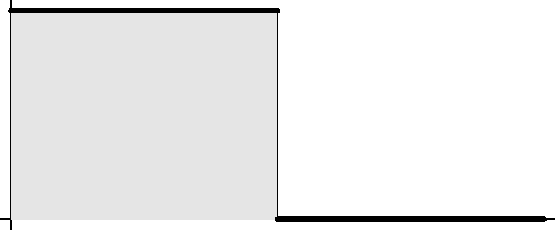
\includegraphics[width=0.45\hsize]{images/w-2}
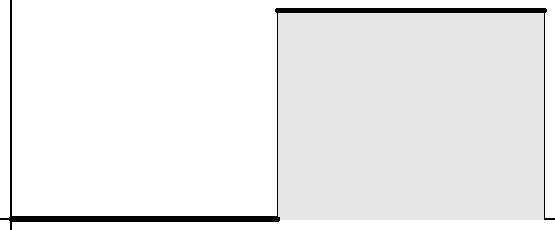
\includegraphics[width=0.45\hsize]{images/w-3}
\end{center}
\caption{Basisfunktionen $\varphi_{1,0}$ und $\varphi_{1,1}$\label{wavelet-phi10-11}}
\end{figure}

Es ist klar, dass man mit diesen Vektoren jedes beliebige Signal
darstellen kann, denn es ist ja
$\varphi_{k,j}=e_j$, die urspr"unglichen Basisvektoren geh"oren 
auch zur Familie der Funktion $\varphi_{i,j}$. Das bedeutet
aber auch, dass $\varphi_{i,j}$ keine Basis sein kann, die Familie
umfasst $2^{k+1}-1$ Vektoren, w"ahrend $V$ nur $2^k$-dimensional ist.

Die Vektoren $\varphi_{i,j}$ sind auch nicht orthogonal. Es ist
zwar $\varphi_{i,j}\cdot\varphi_{i,l}=0$ f"ur $j\ne l$. Aber es
gilt auch $\varphi_{0,0}\cdot\varphi_{i,j}=2^{k-i}$ f"ur jedes
beliebige $j$.

Lineare Abh"angigkeit kommt in der Familie $\varphi_{i,j}$ sehr
h"aufig vor. Bereits die ersten drei Vektoren sind linear
abh"angig:
$$\varphi_{0,0}=\varphi_{1,0}+\varphi_{0,1}.$$
Analoges gilt f"ur beliebige sp"ateren $\varphi$-Vektoren:
$$
\varphi_{i,j}=\varphi_{i+1,2j}+\varphi_{i+1,2j+1}
$$
Insbesondere sind also alle Vektoren $\varphi_{i,j}$ mit 
ungeradem $j$ entbehrlich. F"ur jedes $i>0$ bleiben also
nur noch $2^{i-1}$ Vektoren "ubrig, die linear unabh"angig,
sowie der Vektor $\varphi_{0,0}$. Dies sind
$$
1+\sum_{i=1}^k 2^{i-1}=1+\sum_{i=0}^{k-1}2^i=1+2^{k}-1=2^{k}=N
$$
linear unabh"angige Vektoren.

\subsection{Orthonormierung}
\begin{figure}
\begin{center}
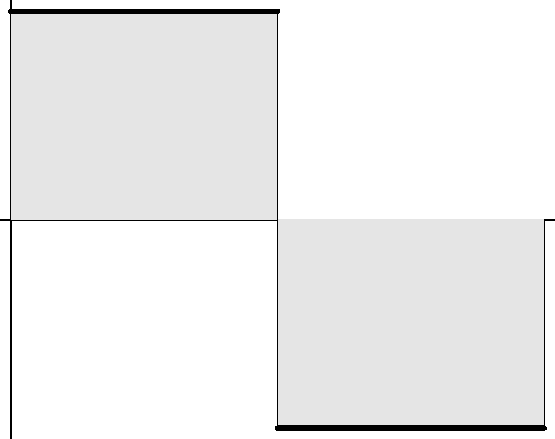
\includegraphics[width=0.45\hsize]{images/w-8}
\end{center}
\caption{Orthogonale Basisfunktion $\psi_{1,0}$\label{wavelet-psi10}}
\end{figure}

Die Vektoren $\varphi_{i,j}$ mit $j$ gerade bilden eine Basis,
mit Hilfe des Orthonormierungs-Algorithmus k"onnen Sie zu einer
orthonormierten Basis gemacht werden. Diesen Prozess verwenden
wir aber nur f"ur die Konstruktion eines ersten Vektors $\psi_{1,0}$,
und leiten daraus dann eine orthonormierte Familie ab.

Der Basisvektor $\varphi_{0,0}$ ist noch nicht
normiert, er hat L"ange $\sqrt{N}$, also ist
$$
\psi_{0,0}=\frac1{\sqrt{N}}\varphi_{0,0}
$$
der erste normierte Basisvektor.

Im zweiten Schritt muss eine Linearkombination von $\psi_{0,0}$
und $\varphi_{1,0}$ gefunden werden, welche L"ange $1$ hat und
auf $\psi_{0,0}$ senkrecht steht. Die Orthogonalit"atsbedingung
kann erf"ullt werden, indem man den Vektor
\[
v=\varphi_{1,0}-(\varphi_{1,0}\cdot\psi_{0,0})\psi_{0,0}
\]
verwendet. Da $\varphi_{1,0}\cdot\psi_{0,0}=\frac{N}2\cdot\frac1{\sqrt{N}}
=\frac1{2\sqrt{N}}$,
ergibt sich
\[
v(l)=\begin{cases}
\frac12&\qquad 0<l\le 2^{k-1}\\
-\frac12&\qquad 2^{k-1}<l\le 2^{k}
\end{cases}
\]
Dieser Vektor h"atte die L"ange $\sqrt{N\frac14}=\frac{\sqrt{N}}2$,
der orthonormalisierte Vektor ist also
\[
\psi_{1,0}=\begin{cases}
\frac1{\sqrt{N}}&\qquad l\le 2^{k-1}\\
-\frac{1}{\sqrt{N}}&\qquad 2^{k-1}<l\le 2^{k},
\end{cases}
\]
siehe auch Abbildung~\ref{wavelet-psi10}.

Mit diesem Vektor kann man jetzt alle Vektoren $\varphi_{1,j}$
darstellen:
\begin{align}
\varphi_{1,0}&=\frac12(\psi_{0,0}+\psi_{1,0})
&
\varphi_{1,1}&=\frac12(\psi_{0,0}-\psi_{1,0})
\label{psikonstruktion}
\end{align}

Jetzt konstruieren wir einen Vektor $\psi_{2,0}$. Wir schreiben $S$
f"ur die Operation des Subsampling:
\[
Sv(l)=\begin{cases}
v(2l)&\qquad 0 <l \le 2^{k-1}\\
0&\qquad 2^{k-1}<l\le N
\end{cases}
\]
Die Operation $S$ nimmt also nur jeden zweiten Wert eines Signals.
Es ist klar, dass $S\varphi_{i,0}=\varphi_{i+1,0}$ und
$S\varphi_{i,1}=\varphi_{i+1,1}$, ebenso bleiben orthogonale
Signale auch nach dem Subsampling orthogonal. Wenden wir dies
auf \ref{psikonstruktion} an, erhalten wir
\begin{align*}
S\varphi_{1,0}&=\frac12(S\varphi_{0,0}+S\psi_{1,0})
&
S\varphi_{1,1}&=\frac12(S\varphi_{0,0}-S\psi_{1,0})
\\
\varphi_{2,0}&=\frac12(\varphi_{1,0}+S\psi_{1,0})
&
\varphi_{2,1}&=\frac12(\varphi_{1,1}-S\psi_{1,0})
\end{align*}
und schliessen ausserdem, das $S\psi_{1,0}$ auf $\varphi_{1,0}$
senkrecht steht. Somit ist $S\psi_{1,0}$ ein guter Kandidat
f"ur $\psi_{2,0}$, nur die L"ange braucht noch nicht zu
stimmen. Da $S\psi_{1,0}$ jedoch f"ur genau die H"alfte der Zeitpunkte
$1$ ist, ist
$$\psi_{2,0}=\sqrt{2}S\psi_{1,0}$$
ein normierte Vektor, der senkrecht auf $\psi_{1,0}$ und $\varphi_{0,0}$
steht, Abbildung~\ref{psi2}.
\begin{figure}
\begin{center}
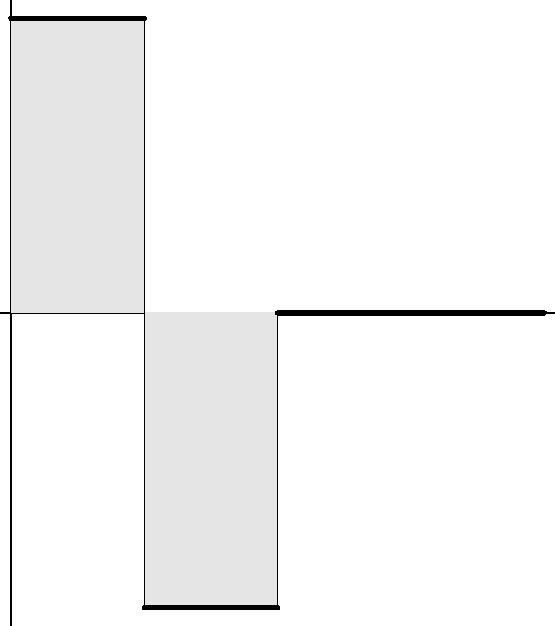
\includegraphics[width=0.45\hsize]{images/w-9}
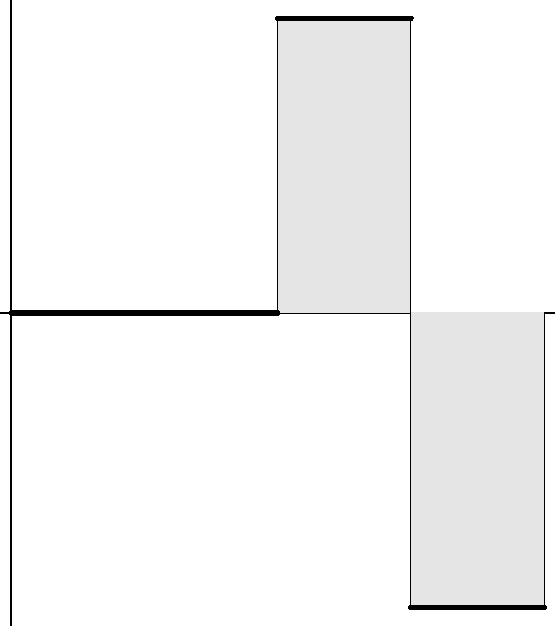
\includegraphics[width=0.45\hsize]{images/w-10}
\end{center}
\caption{Orthogonale Vektoren $\psi_{2,0}$ und $\psi_{2,1}$\label{psi2}}
\end{figure}

\begin{figure}
\begin{center}
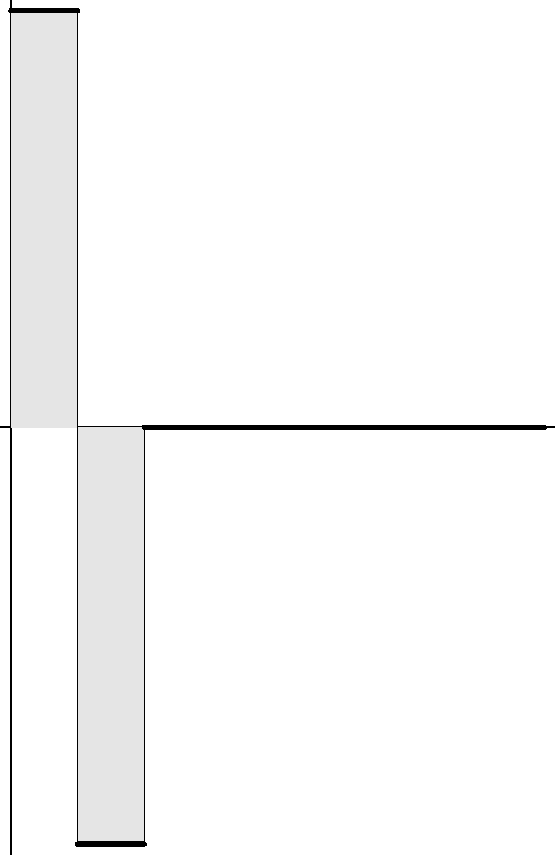
\includegraphics[width=0.22\hsize]{images/w-11}
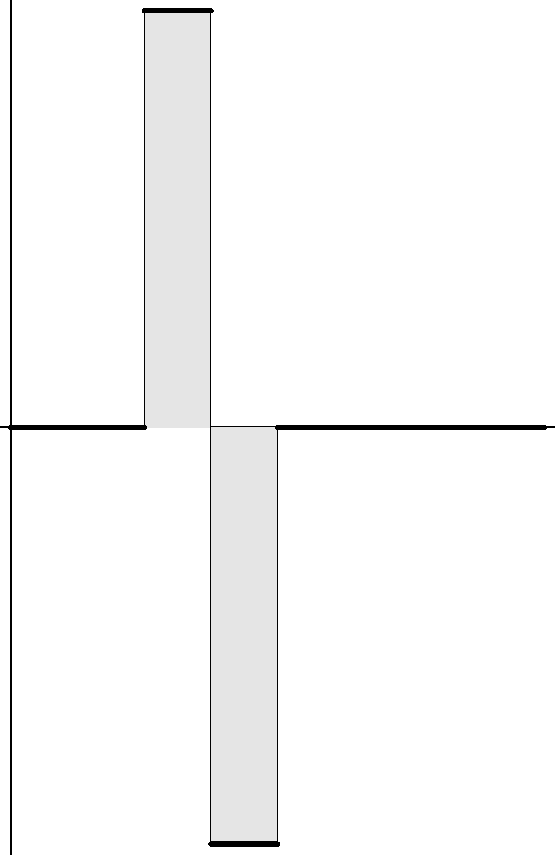
\includegraphics[width=0.22\hsize]{images/w-12}
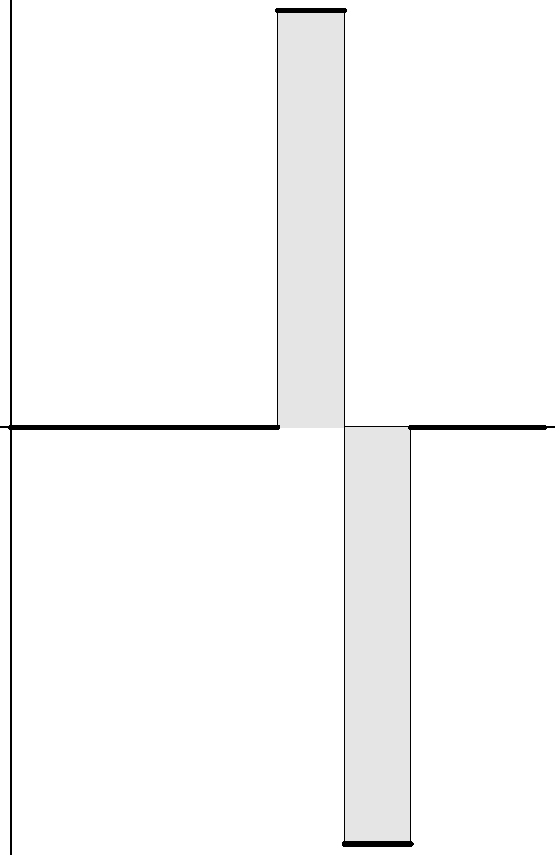
\includegraphics[width=0.22\hsize]{images/w-13}
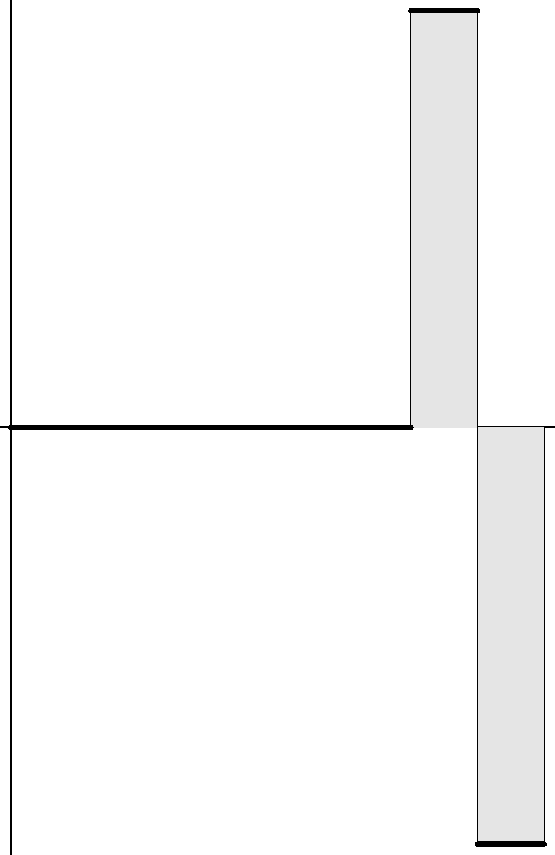
\includegraphics[width=0.22\hsize]{images/w-14}
\end{center}
\caption{Orthogonale Vektoren $\psi_{3,j}$, mit $0\le j\le 3$\label{psi3}}
\end{figure}

Ein weiterer unabh"angiger Vektor kann durch Translation gewonnen werden.
Setzen wir
$$
(T^uv)(l)=\begin{cases}
v(l-v+N)&\qquad l\le v\\
v(l-v)&\qquad l>v\\
\end{cases}
$$
f"ur die Translation um $u$ Stellen, dann ist
$$\psi_{2,1}=T^{2^{k-1}}\psi_{2,0}$$ 
ebenfalls ein Einheitsvektor und orthonormiert, das Resultat ist in Abbildung
\ref{psi2} dargestellt.

Analog kann man f"ur $\psi_{3,j}$ mit $0\le j\le 3$ vorgehen, und
erh"alt vier orthogonale Vektoren wie in Abbildung \ref{psi3}.

\subsection{Analyse}
Da die Vektoren $\psi_{i,j}$ mit $0\le i\le k$ und
$0\le j< 2^i$ eine orthonormierte Basis von $V$ bilden, man kann also
jeden beliebigen Vektor $v$ in dieser Basis zerlegen.
Dazu bildet man die Skalaprodukte
\begin{align*}
a_{i,j}&=\psi_{i,j}\cdot v
\end{align*}
\begin{figure}
\begin{center}
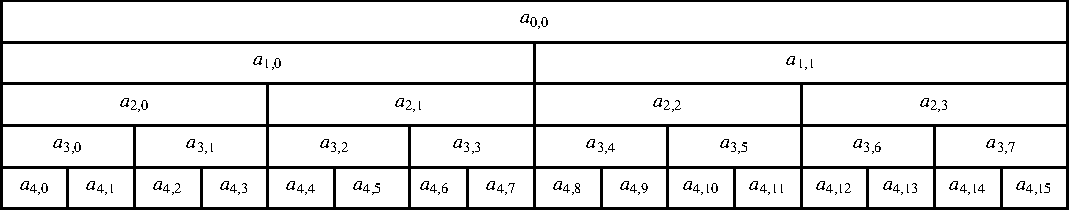
\includegraphics[width=\hsize]{images/signal-4}
\end{center}
\caption{Hierarchie der Koeffizienten $a_{i,j}$\label{coefhierarchy}}
\end{figure}
Die Berechnung der Koeffizienten ist sehr effizient m"oglich, weil die
verschiedenen Funktionen $\psi_{i,j}$ f"ur das selbe $i$ nicht gleichzeitig
von Null verschieden sind, Abbildung~\ref{coefhierarchy}.
Der Koeffizient $a_{0,0}$ ist massgebend f"ur das ganze Zeitintervall,
doch $a_{1,0}$ und $a_{1,1}$ sind je nur f"ur die H"alfte des Intervalls
relevant, und brauchen auch nur Daten aus jeweils der H"alfte
des Intervalls. $a_{i,j}$ wird aus Daten aus einem $2^i$-tel des
Intervalls berechnet.
Die Anforderung, dass die Analyse ``lokale Detailinformation''
liefern soll, ist damit erf"ullt.

\begin{figure}
\begin{center}
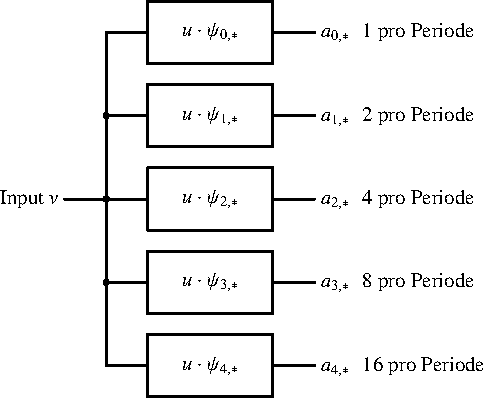
\includegraphics[width=0.65\hsize]{images/signal-2}
\end{center}
\caption{Analyse des Inputsignals $v$ mit der Basis $\{\psi_{i,j}\}$
\label{waveletanalysis}}
\end{figure}
Um den Koeffizienten von $\psi_{i,0}$ zu berechnen wird zuerst
die Summe der ersten $2^{k-i}$ Werte gebildet, dann werden die
n"achsten $2^{k-i}$ Werte subtrahiert, womit die Berechnung von $a_{i,0}$
abgeschlossen ist. Mit den nachfolgenden $2^{k-i+1}$ Werten kann dann
$a_{i,1}$ nach dem gleichen Muster berechnet werden. Mit $k$ parallelen
Recheneinheiten (Abbildung~\ref{waveletanalysis}),
die in jedem Zyklus eine Multiplikation und eine Addition zur
Bildung des Skalarproduktes durchf"uhren k"onnen\footnote{Solche 
Einheiten stehen in FPGAs als Hardwarebl"ocke zur Verf"ugung. Ebenso
implementieren Signalprozessoren genau diese Art von Operation
mit einer einzigen Instruktion.
Die Anzahl pro Sekunde ausf"uhrbarer solcher
Multiply-Accumulate-Operationen (MACs)
ist ein Leistungsmerkmal von FPGAs oder Signalprozessoren.
Man darf also davon ausgehen,
dass diese Art von Berechnung besonders effizient in angepasster
Hardware ausf"uhrbar ist, ganz im Gegensatz zum L"osen eines
Gleichungssystems.}
k"onnen also die Koeffizienten $a_{i,j}$ mit h"ochstens
einem Zyklus Verz"ogerung berechnet werden.

Der Koeffizient von $\psi_{0,0}=\varphi_{0,0}$ berechnet
den Durchschnittswert des Signals, den ``DC-Anteil''.
Der Koeffizient von $\psi_{1,0}$ gibt an, wie gross der Unterschied 
zwischen dem Durchschnittswert der beiden H"alften der Werte
des Signals sind.
Die Koeffizienten $\psi_{i,j}$ geben an, wie stark sich die Mittelwerte
von $2^{k-i}$ aufeinanderfolgenden Werten unterscheiden.
F"ur kleines $i$ werden also Mittelwerte grosser Intervalle
gebildet, und damit hochfrequente Schwankungen ausgemittelt.
Die verschiedenen Koeffizienten $a_{i,j}$ sind also ein Mass
daf"ur, wie stark verschieden hohe Frequenzen im Signal
vertreten sind. Trotzdem geht die Information nicht verloren,
wann eine Signal"anderung passiert.

\subsection{Synthese}
\begin{figure}
\begin{center}
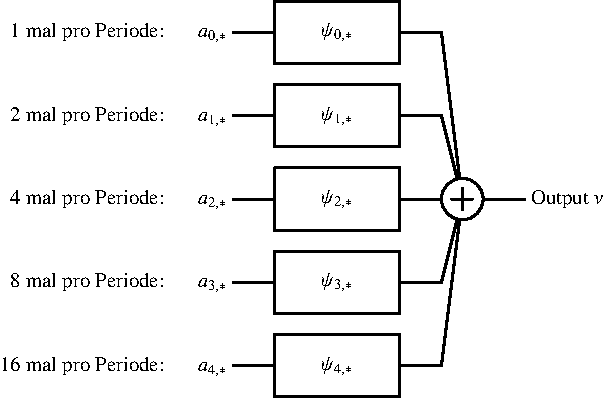
\includegraphics[width=0.8\hsize]{images/signal-3}
\end{center}
\caption{Synthese des Signals $v$ aus den Koeffizienten $a_{i,j}$
\label{waveletsynthesis}}
\end{figure}
Das urspr"ungliche Signal kann aus den Koeffizienten zur"uckgewonnen werden,
indem die Summe
$$
v=a_{0,0}\varphi_{0,0}+\sum_{i=1}^k\sum_{j=0}^{2^i-1}a_{i,j}\psi_{i,j}
$$
gebildet wird. 
Auch diese Summe kann sehr effizient summiert werden, weil zu jedem
Zeitpunkt nur $k$ der Vektoren $\varphi_{0,0}$ und $\psi_{i,j}$
von Null verschieden sind.
Man braucht daher nur f"ur jedes $i$ einen Generator, der
nacheinander die Signale $\psi_{i,j}$ erzeugen kann. "Uber
einen Input, auf den man die Koeffizienten $a_{i,j}$ geben
kann, steuert man die Amplitude der $\psi_{i,j}$-Komponente.
\begin{figure}
\begin{tabular}{|c|c|c|c|}
\hline
\multicolumn{4}{|c|}{
\includegraphics[width=0.22\hsize]{images/w-1}}\\
\hline
\multicolumn{4}{|c|}{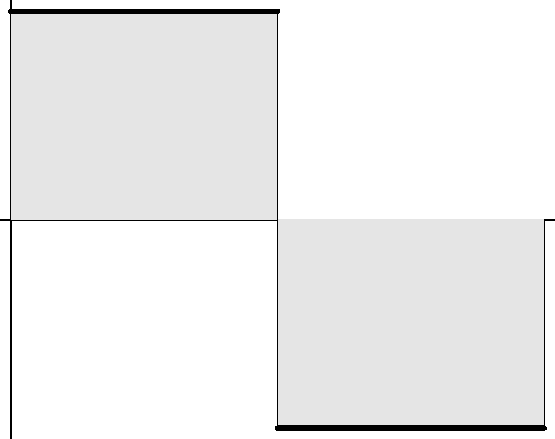
\includegraphics[width=0.22\hsize]{images/w-8}}\\
\hline
\multicolumn{2}{|c|}{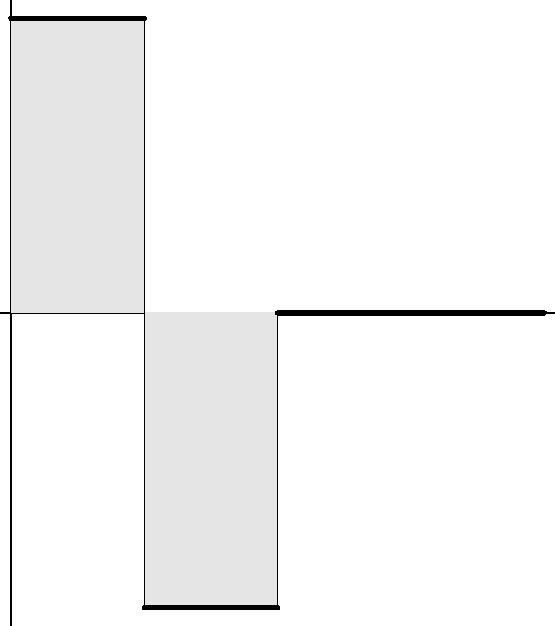
\includegraphics[width=0.22\hsize]{images/w-9}}&%
\multicolumn{2}{|c|}{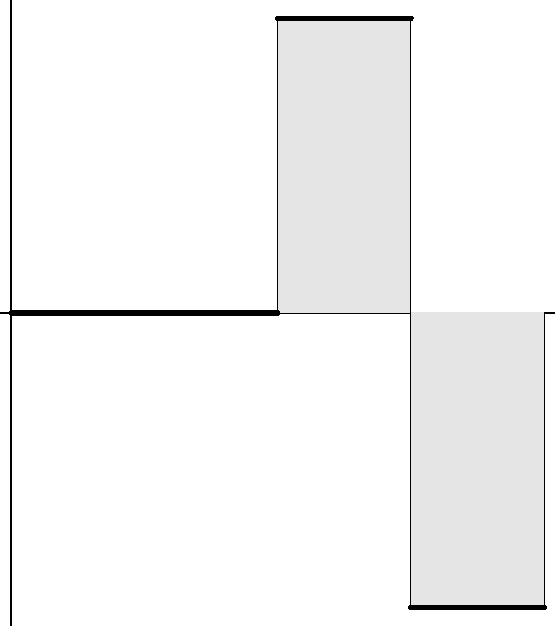
\includegraphics[width=0.22\hsize]{images/w-10}}\\
\hline
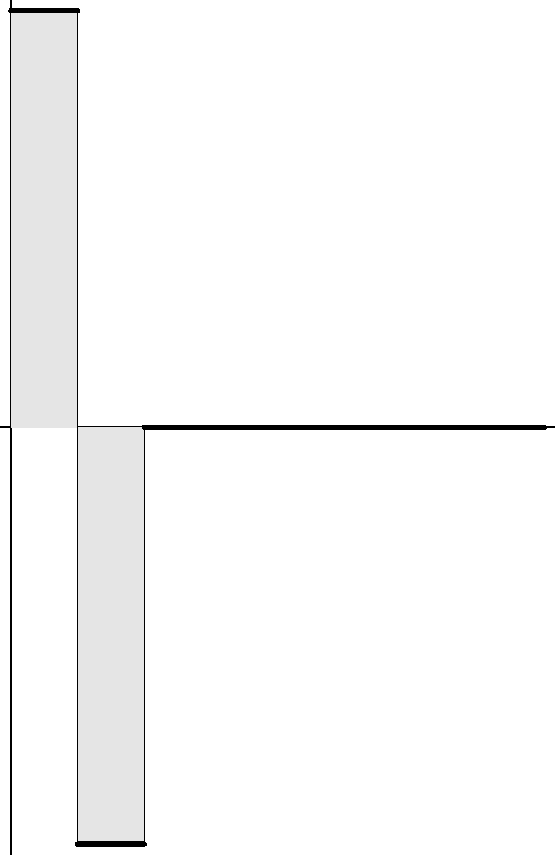
\includegraphics[width=0.22\hsize]{images/w-11}&%
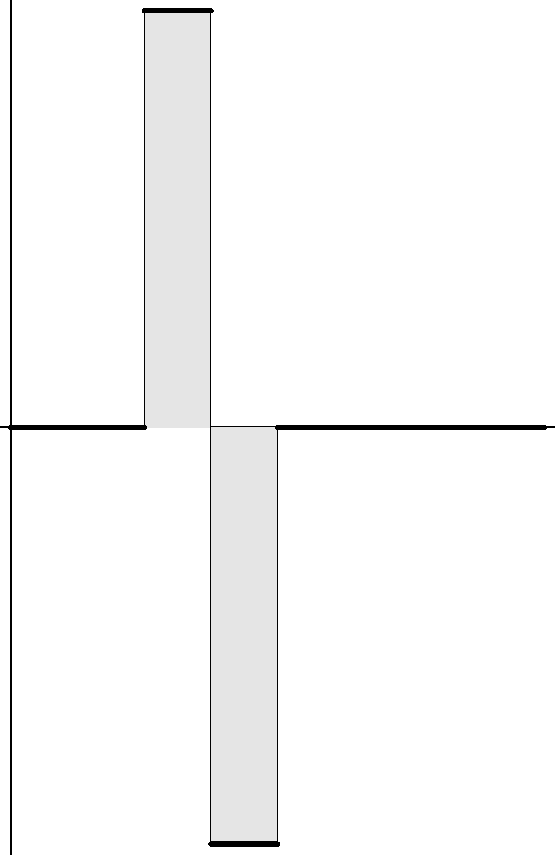
\includegraphics[width=0.22\hsize]{images/w-12}&%
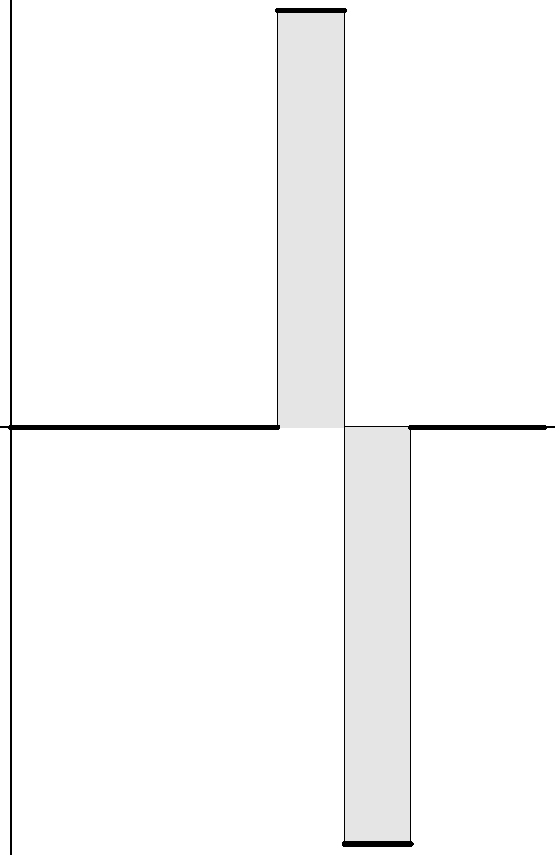
\includegraphics[width=0.22\hsize]{images/w-13}&%
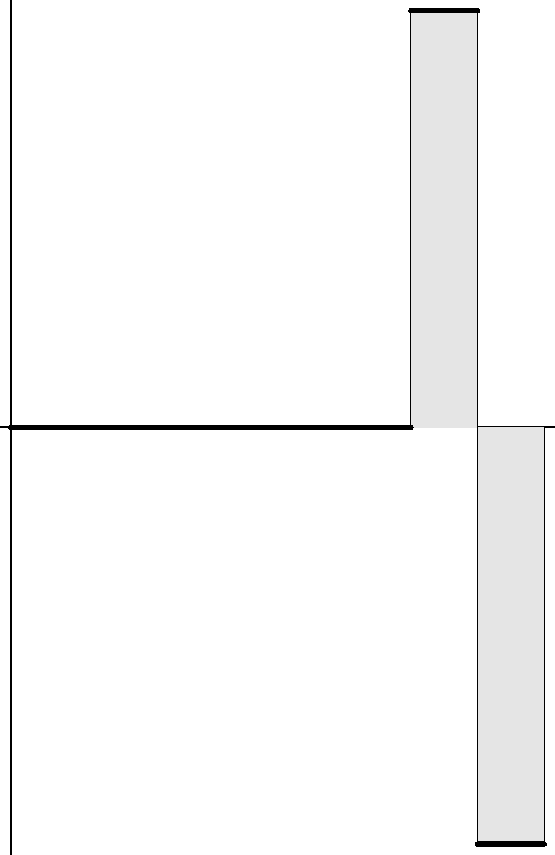
\includegraphics[width=0.22\hsize]{images/w-14}\\
\hline
\end{tabular}
\caption{Die Basisfunktionen $\psi_{i,j}$, $0\le i\le 3$ und $0\le j<2^{i-1}$.}
\end{figure}

\subsection{Wavelet Transformation}
Das Resultat der Analyse ist ein Vektor bestehend aus den Koeffizienten
$a_{i,j}$:
$$
{\cal W}v=\begin{pmatrix}a_{0,0}\\a_{1,0}\\a_{2,0}\\a_{2,1}\\\vdots\end{pmatrix},
$$
die sogenannte Wavelet Transformation von $v$.
Diese Transformation ist linear, f"ur zwei Signale $u$ und $v$ gilt also
\begin{align*}
{\cal W}(u+v)&={\cal W}u+{\cal W}v\\
{\cal W}(\lambda v)&=\lambda{\cal W}v
\end{align*}
Die Synthese zeigt, dass ${\cal W}$ auch umkehrbar ist, es gibt also
eine lineare Transformation ${\cal W}^{-1}$ mit
\begin{align*}
{\cal W}^{-1}{\cal W}v&=v
&
{\cal W}{\cal W}^{-1}a&=a
\end{align*}
Selbstverst"andlich kann man f"ur $\cal W$ auch eine Matrix angeben:
$$
{\cal W}
=
\frac1{\sqrt{N}}
\begin{pmatrix}
1&\dots&1&1&\dots&1&1\\
1&\dots&1&-1&\dots&-1&-1\\
\sqrt{2}&\dots&-\sqrt{2}&0&\dots&0&0\\
0&\dots&0&\sqrt{2}&\dots&-\sqrt{2}&-\sqrt{2}\\
\vdots&\ddots&\vdots&\vdots&\ddots&\vdots&\vdots\\
0&\dots&0&0&\dots&\sqrt{\frac{N}2}&-\sqrt{\frac{N}2}
\end{pmatrix}
$$
Ihre Zeilen enthalten genau die Komponenten der Vektoren
$\varphi_{0,0}$, $\psi_{i,j}$.
Die Matrix der Umkehrtransformation enth"alt dagegen die
Komponenten der Vektoren in den Spalten, also
$$
{\cal W}^{-1}
=
\frac1{\sqrt{N}}
\begin{pmatrix}
1&1&\sqrt{2}&0&\dots&0\\
\vdots&\vdots&\vdots&\vdots&\ddots&\vdots\\
1&1&-\sqrt{2}&0&\dots&0\\
1&-1&0&\sqrt{2}&\dots&0\\
\vdots&\vdots&\vdots&\vdots&\ddots&\vdots\\
1&-1&0&-\sqrt{2}&\dots&\sqrt{\frac{N}2}\\
1&-1&0&-\sqrt{2}&\dots&-\sqrt{\frac{N}2}
\end{pmatrix}
$$

\subsection{Anwendungen}
\begin{figure}
\begin{center}
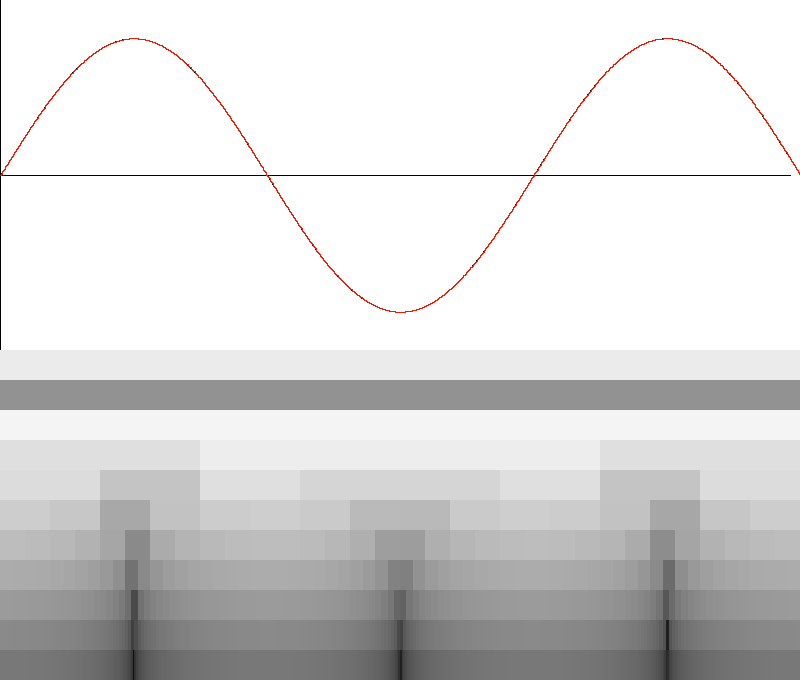
\includegraphics[width=\hsize]{graphics/wavelet-sin3}
\end{center}
\caption{Haar-Wavelet-Transformation eines Sinus-Signals. Oben das Signal,
unten die Koeffizienten $a_{i,j}$ in logarithmischer Darstellung.
Absolut kleine Koeffizienten werden dunkel dargestellt, Koeffizienten
mit grossem Absolutwert dagegen hell.\label{wavelet-sin}}
\end{figure}
\begin{figure}
\begin{center}
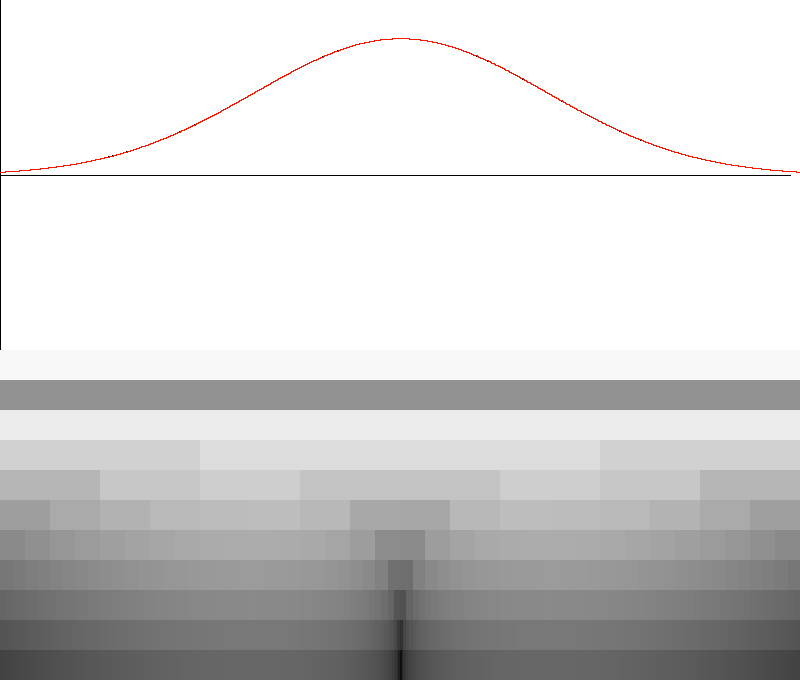
\includegraphics[width=\hsize]{graphics/wavelet-normal}
\end{center}
\caption{Haar-Wavelet-Transformation eines Gauss-Signals. Siehe 
auch Bildlegende zu Abbildung~\ref{wavelet-sin}\label{wavelet-normal}}
\end{figure}
Die Abbildungen \ref{wavelet-sin} und \ref{wavelet-normal} zeigen
die Koeffizienten $a_{i,j}$ f"ur ein Sinus-Signal und f"ur ein
ein Gauss-Signal. Da die h"oheren Koeffizienten vor allem den
Unterschied zwischen benachbarten Teilintervallen feststellen,
f"allt sofort auf, dass die h"oheren Koeffizienten in der
N"ahe der Extrema besonders klein werden.
Dagegen misst $a_{0,0}$ den Mittelwert, also das Integral des Signals.

Man kann die Wavelet Transformation zum Beispiel f"ur die Signalkomprimierung
brauchen. Nat"urliche Signale werden nicht zu schnell ansteigen, die
Koeffizienten $a_{i,j}$ f"ur $i=k-1$, welche die Zu- oder Abnahme des
Signals von Messpunkt zu Messpunkt angeben, werden also eher klein
sein. Es ist daher m"oglich, sie mit einer geringeren Anzahl von Bits
zu codieren, oder sogar ganz wegzulassen, und damit Speicherplatz zu
sparen. Nach diesem Prinzip funktioniert zum Beispiel die JPEG Komprimierung.

Nat"urlich geht durch das Weglassen von Komponenten Information verloren.
Dies wird zum Beispiel dazu verwendet, um Personen auf Bildern unkenntlich
zu machen. L"asst man alle hohen Komponenten weg, bleibt vom Signal
nur noch eine grobe Treppenfunktion "ubrig.
"Ubersetzt auf ein zweidimensionales Bild, heisst dies, dass nur noch
ein grobes Pixelraster "ubrig bleibt, auf dem eine Person nicht mehr
erkennbar ist.

Das Weglassen von hohen Komponenten kann ebenfalls mit einer Matrix
beschrieben werden:
$$
P=\begin{pmatrix}
1&\dots&0&0&\dots&0\\
\vdots&\ddots&\vdots&\vdots&\ddots&\vdots\\
0&\dots&1&0&\dots&0\\
0&\dots&0&0&\dots&0\\
\vdots&\ddots&\vdots&\vdots&\ddots&\vdots\\
0&\dots&0&0&\dots&0\\
\end{pmatrix}
$$
Der Filter, der die hochfrequenten Koeffizienten unterdr"uckt kann
also wie folgt berechnet werden:
$$
v_{\text{gefiltert}}={\cal W}^{-1}P{\cal W}v.
$$
Umgekehrt kann man die hohen Koeffizienten verst"arken. In Bildern tut
man dies zum Beispiel, um Kanten  stärker hervortreten zu lassen.
Will man die hohen Koeffizienten mit dem Faktor $\lambda$ verst"arken,
kann man dies mit dem Filter
$$
v_{\text{enhanced}}={\cal W}^{-1}(P + \lambda(I-P)){\cal W}v
$$
tun.
